\documentclass[12pt,thmsa]{article}\usepackage[]{graphicx}\usepackage[]{color}
% maxwidth is the original width if it is less than linewidth
% otherwise use linewidth (to make sure the graphics do not exceed the margin)
\makeatletter
\def\maxwidth{ %
  \ifdim\Gin@nat@width>\linewidth
    \linewidth
  \else
    \Gin@nat@width
  \fi
}
\makeatother

\definecolor{fgcolor}{rgb}{0.345, 0.345, 0.345}
\newcommand{\hlnum}[1]{\textcolor[rgb]{0.686,0.059,0.569}{#1}}%
\newcommand{\hlstr}[1]{\textcolor[rgb]{0.192,0.494,0.8}{#1}}%
\newcommand{\hlcom}[1]{\textcolor[rgb]{0.678,0.584,0.686}{\textit{#1}}}%
\newcommand{\hlopt}[1]{\textcolor[rgb]{0,0,0}{#1}}%
\newcommand{\hlstd}[1]{\textcolor[rgb]{0.345,0.345,0.345}{#1}}%
\newcommand{\hlkwa}[1]{\textcolor[rgb]{0.161,0.373,0.58}{\textbf{#1}}}%
\newcommand{\hlkwb}[1]{\textcolor[rgb]{0.69,0.353,0.396}{#1}}%
\newcommand{\hlkwc}[1]{\textcolor[rgb]{0.333,0.667,0.333}{#1}}%
\newcommand{\hlkwd}[1]{\textcolor[rgb]{0.737,0.353,0.396}{\textbf{#1}}}%
\let\hlipl\hlkwb

\usepackage{framed}
\makeatletter
\newenvironment{kframe}{%
 \def\at@end@of@kframe{}%
 \ifinner\ifhmode%
  \def\at@end@of@kframe{\end{minipage}}%
  \begin{minipage}{\columnwidth}%
 \fi\fi%
 \def\FrameCommand##1{\hskip\@totalleftmargin \hskip-\fboxsep
 \colorbox{shadecolor}{##1}\hskip-\fboxsep
     % There is no \\@totalrightmargin, so:
     \hskip-\linewidth \hskip-\@totalleftmargin \hskip\columnwidth}%
 \MakeFramed {\advance\hsize-\width
   \@totalleftmargin\z@ \linewidth\hsize
   \@setminipage}}%
 {\par\unskip\endMakeFramed%
 \at@end@of@kframe}
\makeatother

\definecolor{shadecolor}{rgb}{.97, .97, .97}
\definecolor{messagecolor}{rgb}{0, 0, 0}
\definecolor{warningcolor}{rgb}{1, 0, 1}
\definecolor{errorcolor}{rgb}{1, 0, 0}
\newenvironment{knitrout}{}{} % an empty environment to be redefined in TeX

\usepackage{alltt}
\usepackage[french,english]{babel}
\usepackage[ansinew]{inputenc}
\usepackage[T1,OT1]{fontenc}
\usepackage{graphicx}
\usepackage{amsmath,amssymb,listings}
\usepackage{alltt,algorithmic,algorithm}
\usepackage{multicol}
\usepackage{cite}
\usepackage{fancyhdr}
\usepackage{setspace}
\usepackage{array}
\usepackage{amsfonts}
\usepackage{latexsym}
\usepackage{epsf}
\usepackage{umlaute}
\usepackage{setspace}
\usepackage{amsthm}
\usepackage{enumerate}


\setlength{\textwidth}{160mm}
\setlength{\textheight}{230mm}
\setlength{\oddsidemargin}{-5mm}
\setlength{\topmargin}{-10mm}

% to get rid of the numbers in the bibliography:
\makeatletter
\def\@biblabel#1{}
\makeatother



\title{Assignement 8}
\IfFileExists{upquote.sty}{\usepackage{upquote}}{}
\begin{document}


\noindent \textsc{University of Geneva}     \hfill \textsc{Bachelor in Economics and Management} \\
\textbf{Probability 1}                      \hfill \textsc{Bachelor in International Relations} \\
Dr. Daniel \textsc{Flores Agreda}                 \hfill Spring 2021  \\
ASSIGNMENT 08                               \hfill   April 23th-27th



\noindent
\makebox[\linewidth]{\rule{\textwidth}{0.4pt}}\\[1.5ex]

\section*{Exercise 1}
%\begin{figure}[thb]
%\label{continu}
\centerline{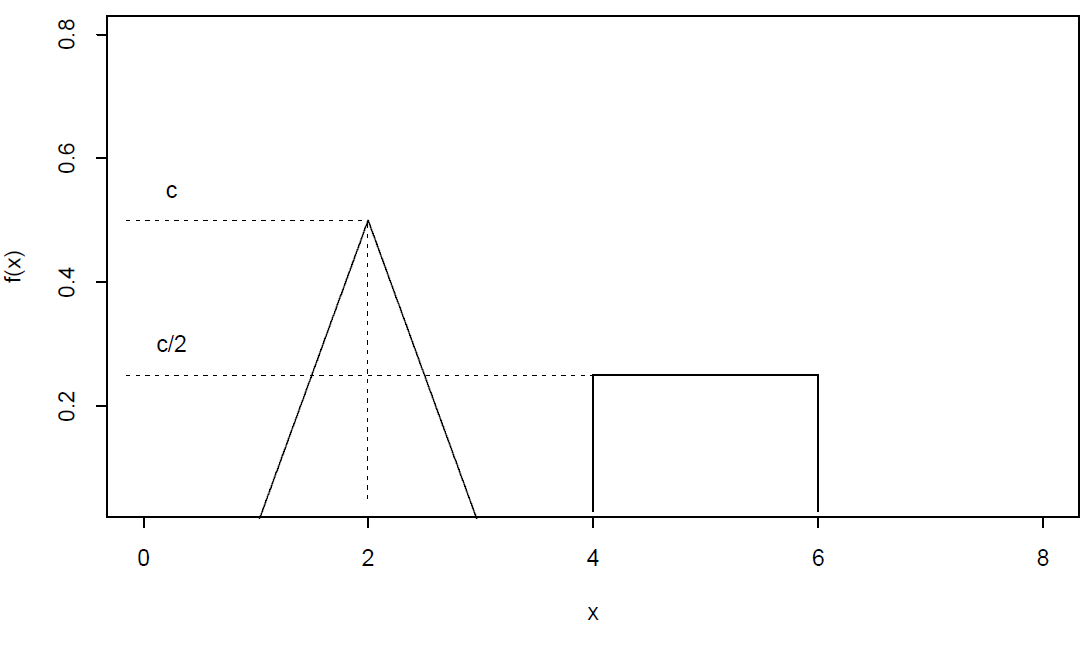
\includegraphics[height=9cm]{figure.png}}
%% \centerline{\epsfig{figure=continu.eps,height=7cm}}
%\caption{ Fonction de densit\'e}
%\end{figure}
\bigskip

\begin{enumerate}%[(a)]
\item Determine the value of c so that the function $f(x)$ in the figure above is a density function. % \ref{continu}

\item Determine the density function $f(x)$.
\item Calculate E$(X)$.
% \item Quelle est la valeur prise par la m\'ediane? Est-elle unique? Expliquer.
\item Determine $P(X \geq 2)$, $P(X \leq 4.5)$ and $P(2.5 \leq X \leq
5)$.
\end{enumerate}





\section*{Exercise 2}

You arrive at a bus stop knowing that the waiting time is a random variable uniformly distributed between 0 and 30 minutes.

\medskip

\noindent The density function of this variable is written as:
 $$
 f (t) = \left\{ \begin{array}{cl}
 0 , & t \le 0;\\
 {1\over 30} , & 0 < t < 30;\\
 0 , & t \ge 30.
 \end{array} \right.
 $$
\smallskip

 \begin{enumerate}%[(a)]
 \item Determine the distribution function $F(t)$ of this variable.
 \item What is the probability that you have to wait more than 10 minutes.
 \item If after 15 minutes' waiting the bus has not arrived yet, what is the probability that you have to wait at least 10 more minutes?
 \end{enumerate}



\section*{Exercise 3}


Let $Z$ be a random variable with the following distribution function:
$$
F(z)=k z^{3} \left (\frac{1}{3} - \frac{z}{2} + \frac{z^{2}}{5} \right ), \ \ 0 \leq z \leq 1,
$$
with $k$ a positive constant.
\medskip

\begin{enumerate}%[(a)]
\item {Find the density function of $Z$ as well as the value of $k$.}
\item {Calculate the expectation and variance of $Z$.}
\item {Calculate $P(0.75 < Z < 1.5)$ and $P(Z \geq 0.15)$.}
% \item {La m\'ediane de $Z$ est \'egale \`a 0.5. En comparant la m\'ediane avec l'esp\'erance, que peut-on dire sur la
% sym\'etrie de Z?}
% % \item {Une \'etude a montr\'e que dans un cas pratique $Z$ ne pouvait pas
% % \^etre inf\'erieure \`a 0.25. Trouver la probabilit\'e que $Z$ soit
% sup\'erieure à 0.5 dans ce cas.}
\item Suppose we know in a particular case that Z is not less than 0.25. Find the probability that Z is greater than 0.5 in this case.

\end{enumerate}



\section*{Exercise 4}

The lifetime $X$ in years of a television follows an exponential law with density:
\begin{equation*}
f(x)=\lambda e^{-\lambda x} ,\quad x\geq 0.
\end{equation*}
\begin{enumerate}
  \item Compute the cumulative distribution function $F(x)$.
  \item Compute the $\alpha$-quantile $q_\alpha=F^{-1}(\alpha)$.
  \item The expected life of your television is $8$ years. What is the probability that the lifetime of your television is more than $8$ years ?
  Evaluate the median.
  \item Compute the variance of $X$ for any $\lambda$.
\end{enumerate}


\section*{Exercise 5 (Optional)}
Everyday, Sveta goes to the university by bike and follows the same 15km path. Her speed is a random variable $V$ which depends on the climate and traffic conditions.
Its density has the following form:
\begin{equation*}
f_V(v)= \left\{
    \begin{array}{ll}
        C v \exp(-\lambda v) &  v\geq 0 \\
        0 & otherwise.
    \end{array}
\right.
\end{equation*}

Sveta is really athletic and rides at a speed of 30 km/h in average.
\begin{enumerate}
  \item Determine the values of $C$ and $\lambda$.
  \item The duration of the ride is described by a the variable $T= \frac{15}{V}$.
  Compute the density and the expectation of $T$.
\end{enumerate}











\end{document}



